%Miriam Clustering
The first question was: is it possible without knowing the social classes to reproduce them based on the movement data. Therefore we wanted to look for clusters and compare those with the strata. Also we had a look if the possibly found clusters have special properties.

\subsubsection{Clustering with RapidMiner}

RapidMiner has different Modules for Clustering already implemented. We decided to concentrate on the k-means clustering algorithm.
\begin{figure}[!htbp]
\centering
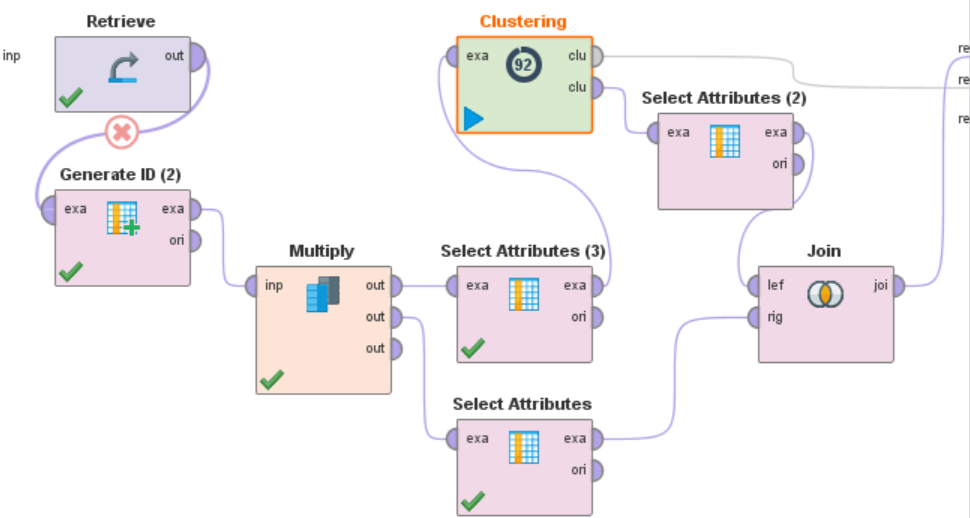
\includegraphics[width=0.9\textwidth]{ClusteringRapid.PNG}
\caption{Process of k-means clustering}
\label{fig: kclust}
\end{figure}


The Process, figure \ref{fig: kclust}, contains the following steps:
\begin{description}
	\item[Retrieve] gives the data into the process. 
  \item[Generate ID] creates an ID such that we can make the comparsion step at the end through joining the sets
  \item[Multiply] creates two identical data sets
  \item[Select Attrbiutes] thoughs away the strata before the clustering step, everything behalve cluster and id after the clustering and just keeps id and strata for the join step
	\item[Clustering] runs the k-means clustering algorithm. The number of Clusters has to be fixed.
	\item[Join] For comparing the clustering result and the strata we join the two filtered data sets by the id
\end{description}

In the clustering block we can chose between different distance measures and maximal step numbers. We decided to concentrate on almost everywhere basic configurations and chose the squared euclidean distance in the mixed version.

In the first step we tried to cluster the \textbf{Original Data} in \textbf{6 Cluster}. Therefore we retrieved the original data set in RapidMiner and chose k as 6.

\ref{fig:OrgDist}. 
\begin{figure}[!htbp]
\centering
\begin{subfigure}{.5\textwidth}
  \centering
  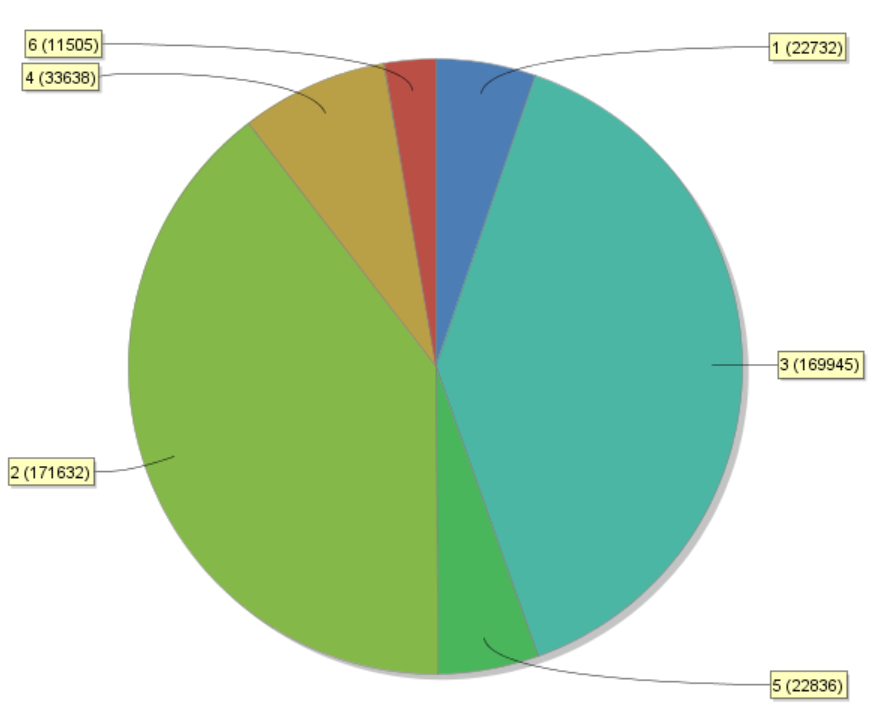
\includegraphics[width=.8\linewidth]{ClusterOrigRapidStrata.PNG}
  \caption{Strata}
  \label{fig:OrgSt}
\end{subfigure}%
\begin{subfigure}{.5\textwidth}
  \centering
  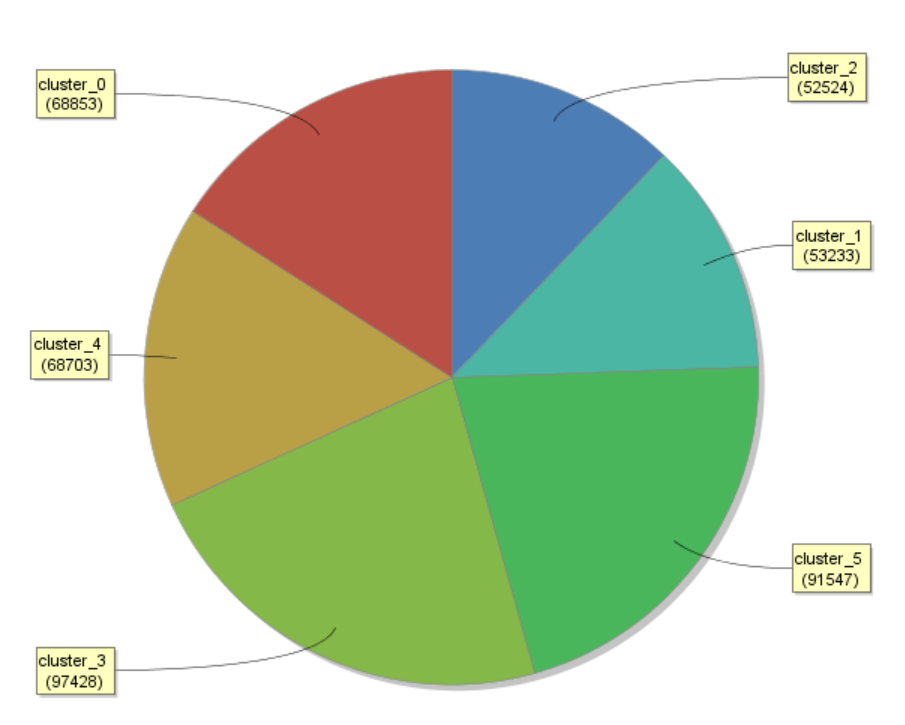
\includegraphics[width=.8\linewidth]{ClusterOrigRapidCluster.PNG}
  \caption{Cluster}
  \label{fig:OrgCl}
\end{subfigure}
\caption{Distribution of original data}
\label{fig:OrgDist}
\end{figure}

In figure \ref{fig:OrgDist} is the result to see of the first try. Figure \ref{fig:OrgSt} shows the strata distribution as pie chart and \ref{fig:OrgCl} the resulted cluster distribution. It can already been seen, that the distributions are not similar. In the next step we tried it with more steps, but the result was not looking better.

We asked ourselfs, if 6 cluster is not too fine, so we searched for \textbf{3 clusters} in the next step. The idea is to combine two stratas in 1, such that we just have 3 stratas left.
\begin{figure}[!htbp]
\centering
\begin{subfigure}{.5\textwidth}
  \centering
  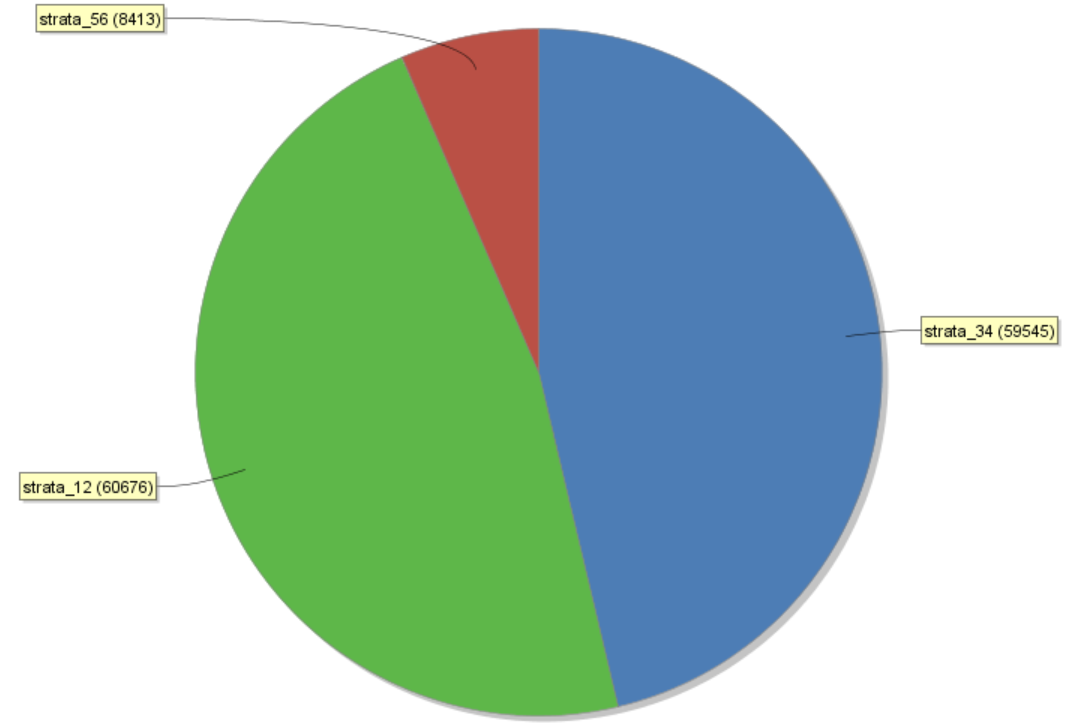
\includegraphics[width=.8\linewidth]{ClusterOrigRapidStrata2Cluster.PNG}
  \caption{Strata}
  \label{fig:OrgSt}
\end{subfigure}%
\begin{subfigure}{.5\textwidth}
  \centering
  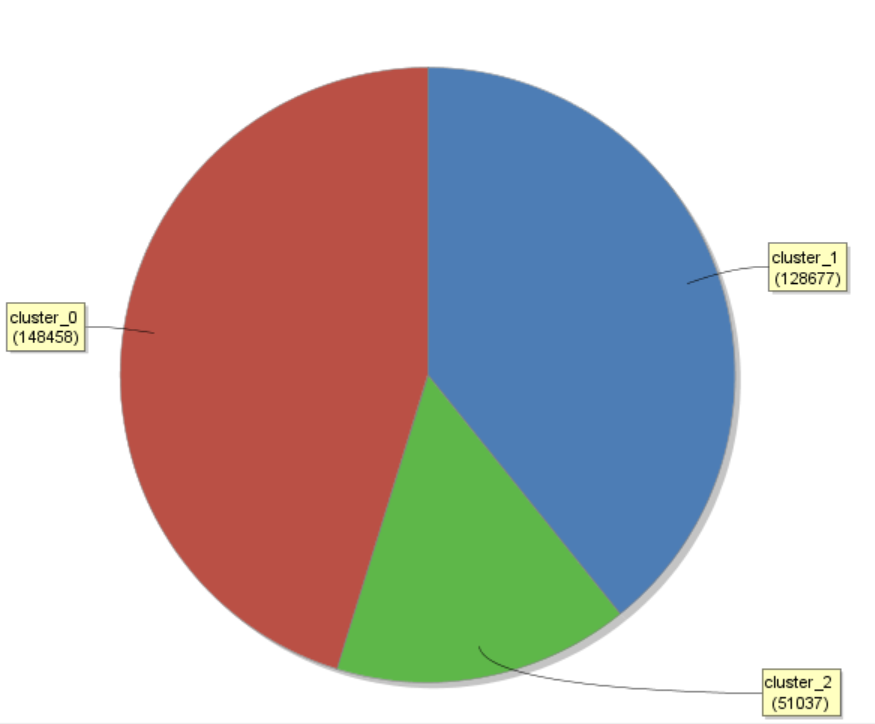
\includegraphics[width=.8\linewidth]{ClusterOrigRapidCluster2Cluster.PNG}
  \caption{Cluster}
  \label{fig:OrgCl}
\end{subfigure}
\caption{Distribution of original data for just 3 clusters}
\label{fig:OrgDist3Cl}
\end{figure}

\begin{figure}[!htbp]
\centering
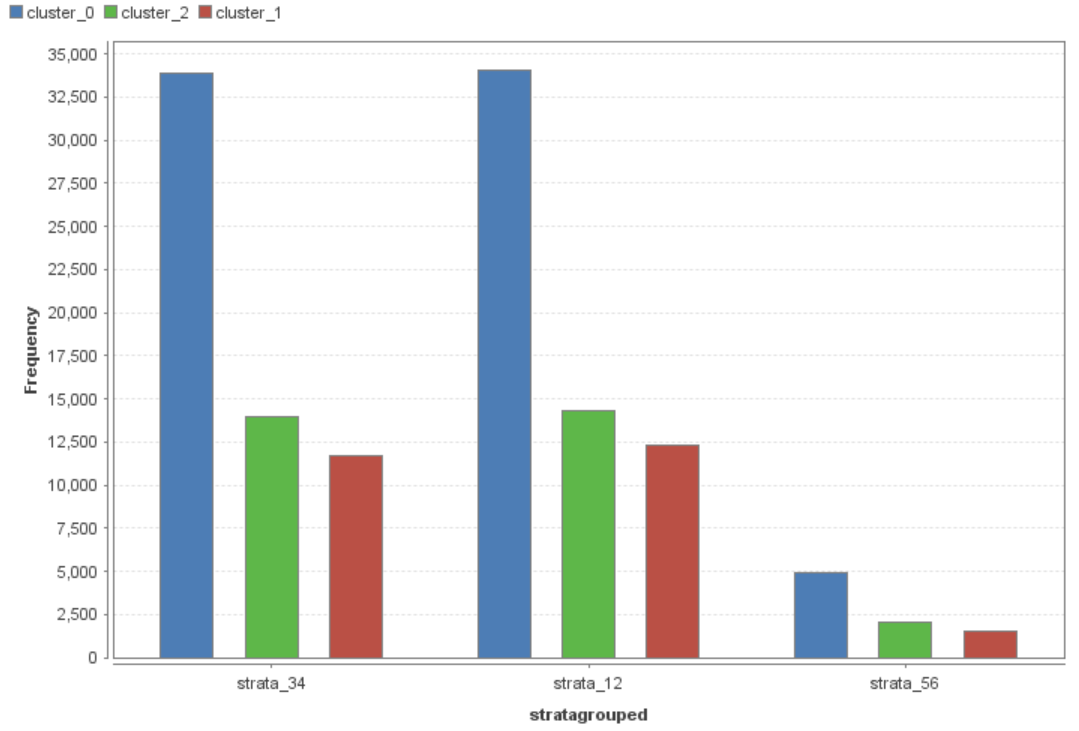
\includegraphics[width=0.9\textwidth]{ClusterOrigRapidDistribution2Cluster.PNG}
\caption{Distribution of the clusters in between the grouped strata}
\label{fig:Groupdist}
\end{figure}

After having a look at the pie charts, \ref{fig:OrgDist3Cl} and so the distribution in between the variable it seems to be a better result, so we had a look at the cluster distribution in the 3 grouped stratas, \ref{fig:Groupdist}. This figure shows clearly, that there is no real correlation between strata 

\begin{figure}[!htbp]
\centering
\begin{subfigure}{0.9\textwidth}
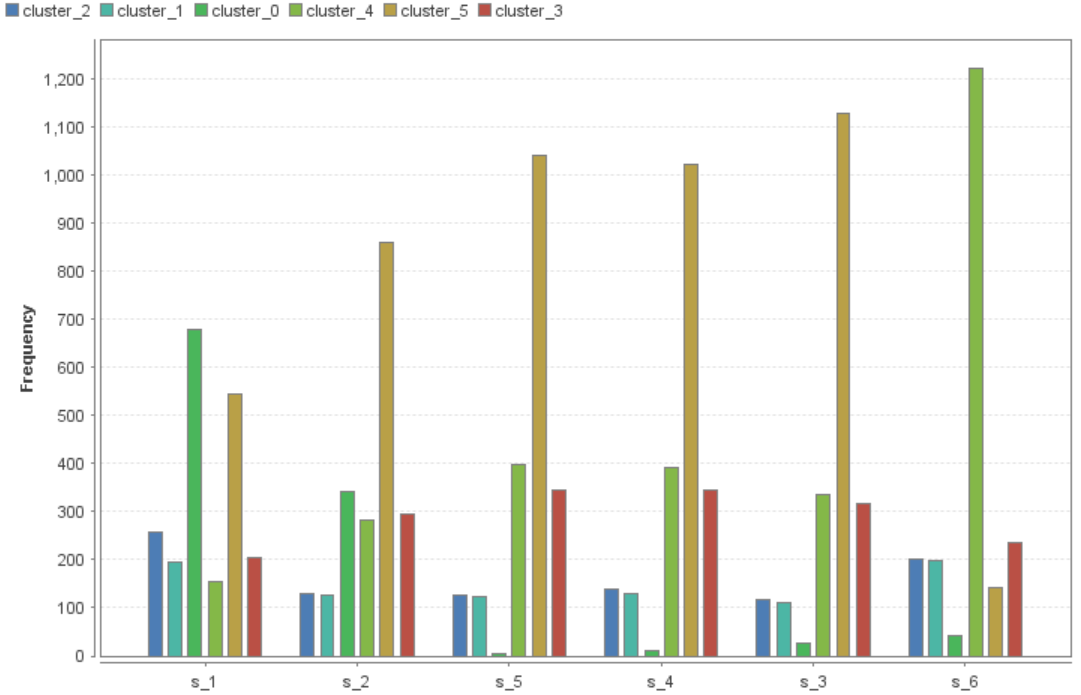
\includegraphics[width=\linewidth]{ClusterOrigRapidDistribution2038eq.PNG}
\caption{For 6 clusters}
\label{fig:2038_6}
\end{subfigure}
\begin{subfigure}{0.9\textwidth}
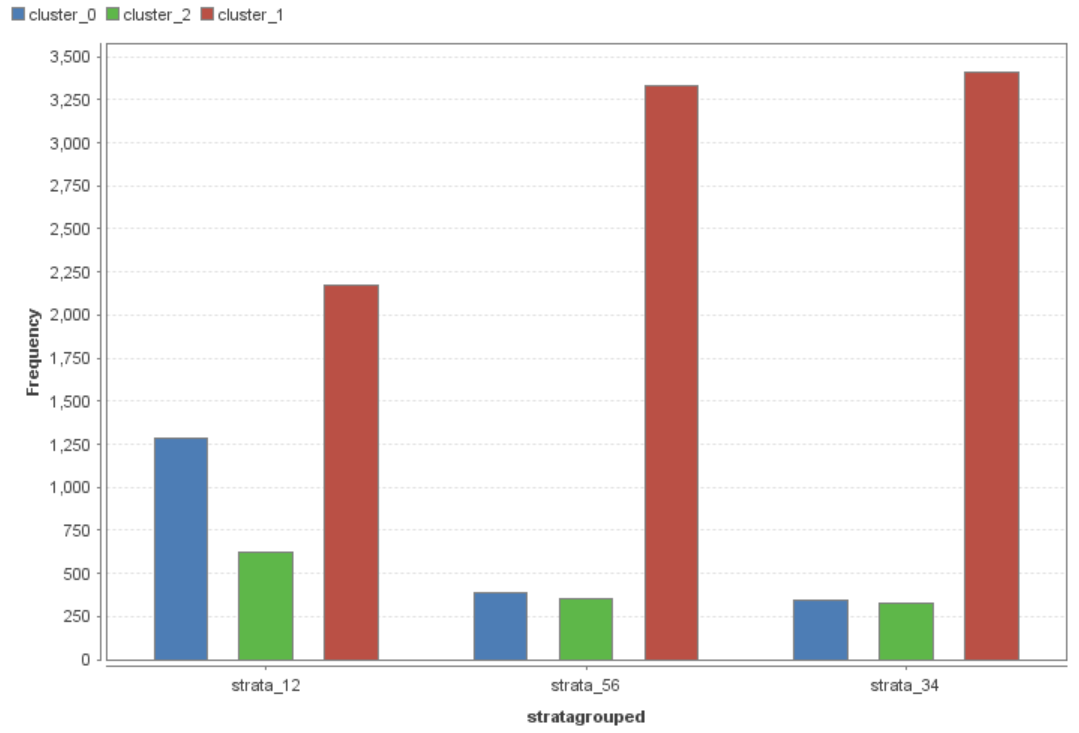
\includegraphics[width=\linewidth]{ClusterOrigRapidDistribution2038eq2.PNG}
\caption{For 3 clusters}
\label{fig:2038_3}
\end{subfigure}
\caption{Distribution of the clusters in between the strata}
\label{fig:2038_Clust}
\end{figure}

The result for different datasizes and equal distribution of the stratas does not change the result. The biggest equal distributed dataset has 2038 data rows for every strata and 4076 in between the grouped strata. In figure \ref{fig:2038_Clust} the two clustering results can be seen. Again we could not really see a significant correlation.

\textbf{Stratified Person Data}

After those not really convincing results we applied the process on the stratified person data, because those represented the movement of one person.

\begin{figure}[h]
\centering
\begin{subfigure}{.5\textwidth}
  \centering
  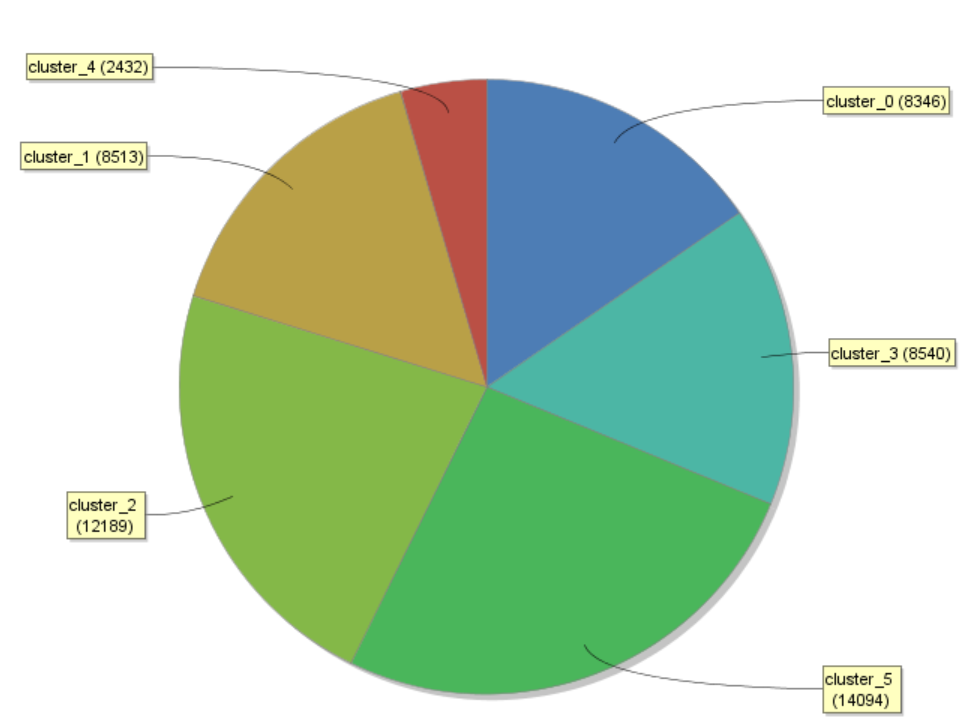
\includegraphics[width=.9\linewidth]{vectorclusteringcluster.PNG}
  \caption{Strata}
  \label{fig:VecSt}
\end{subfigure}%
\begin{subfigure}{.5\textwidth}
  \centering
  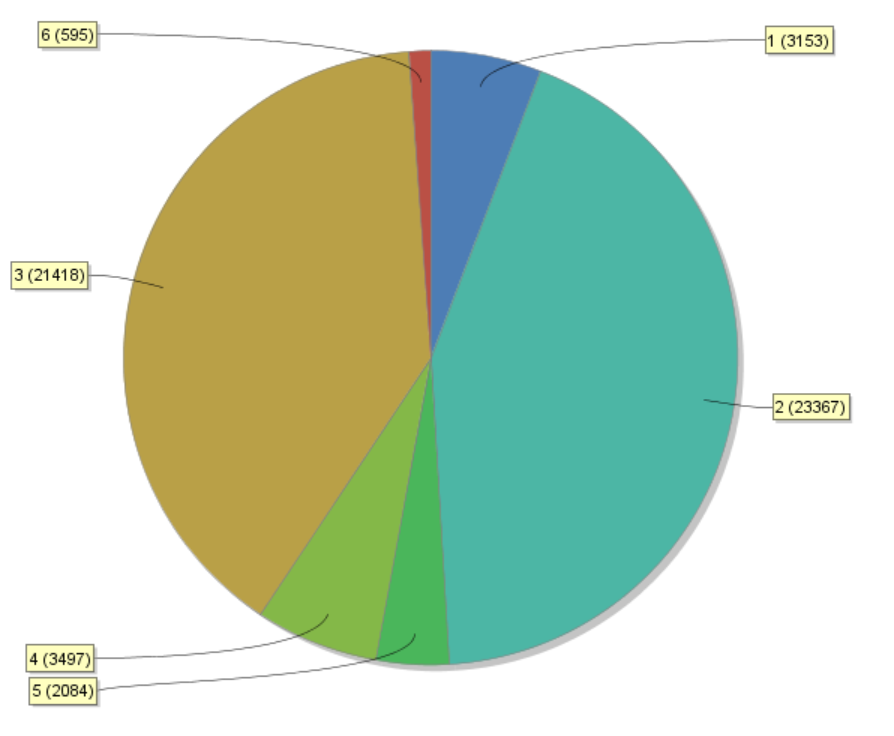
\includegraphics[width=.9\linewidth]{vectorclusteringstrata.PNG}
  \caption{Cluster}
  \label{fig:VecCl}
\end{subfigure}
\caption{Distribution of stratified person data}
\label{fig:VecDist}
\end{figure}

\begin{figure}[!htbp]
\centering
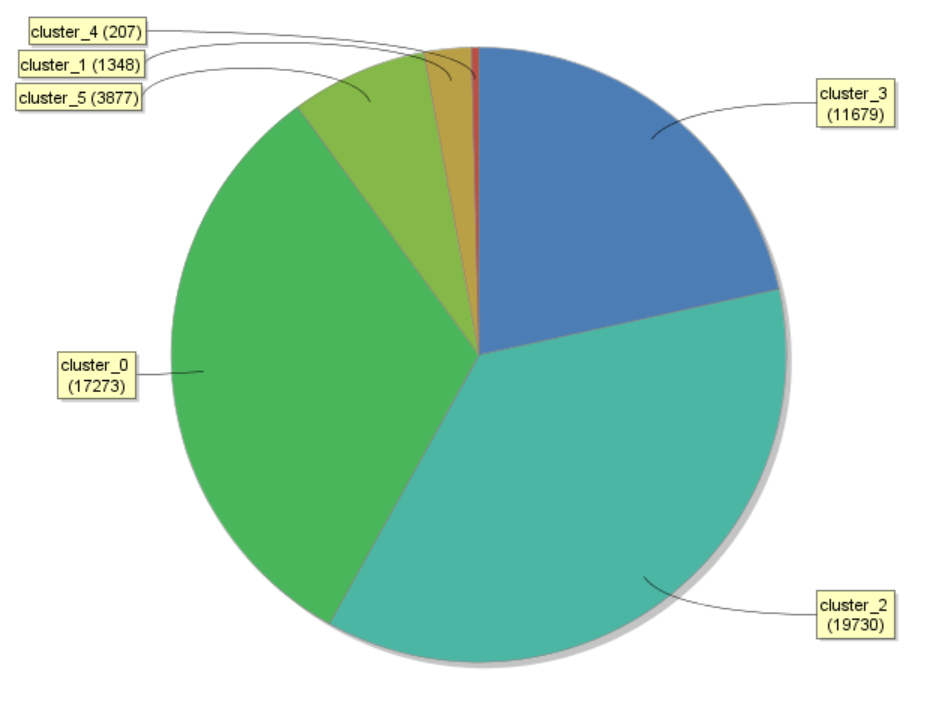
\includegraphics[width=0.3\textwidth]{vectorclusteringcluster1000.PNG}
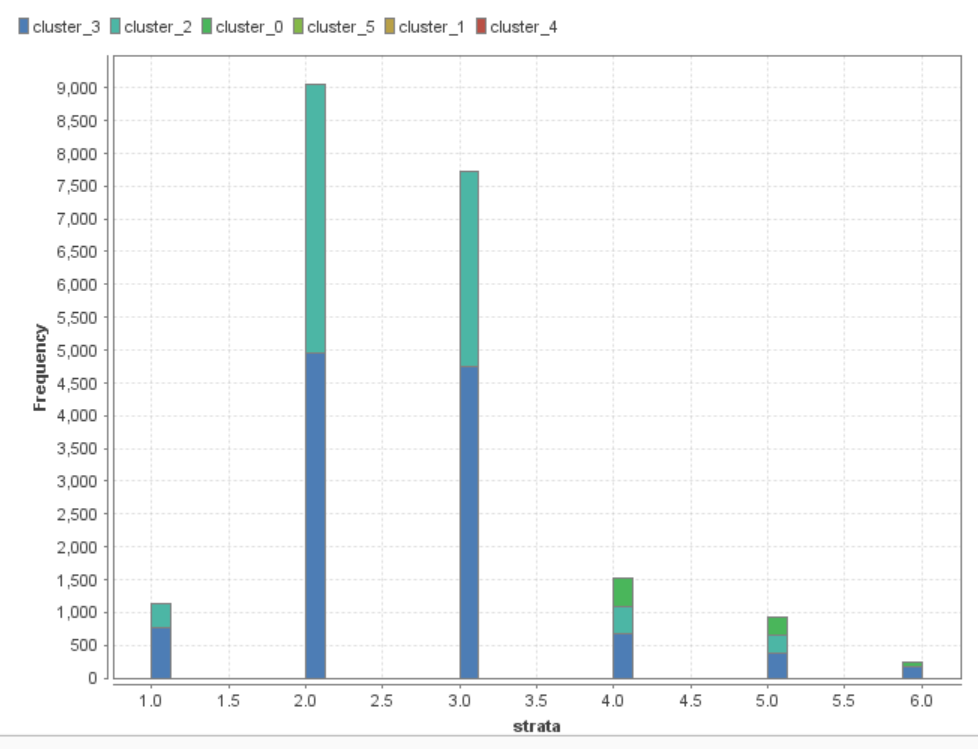
\includegraphics[width=0.69\textwidth]{vectorClustering1000.PNG}
\caption{1000 steps clustering in 6 clusters}
\label{fig:1000vect}
\end{figure}

The results for the whole data set without equalization are shown in figure \ref{fig:2038_Clust}. We changed the number of steps to 1000 for comparsion and the result, \ref{fig:1000vect}, let us assume, that 3 clusters better would fit. 


So we applied the process on the \textbf{stratified person data} and searched for \textbf{3 clusters}. We directly run the algorithm 1000 steps.

\begin{figure}[!htbp]
\centering
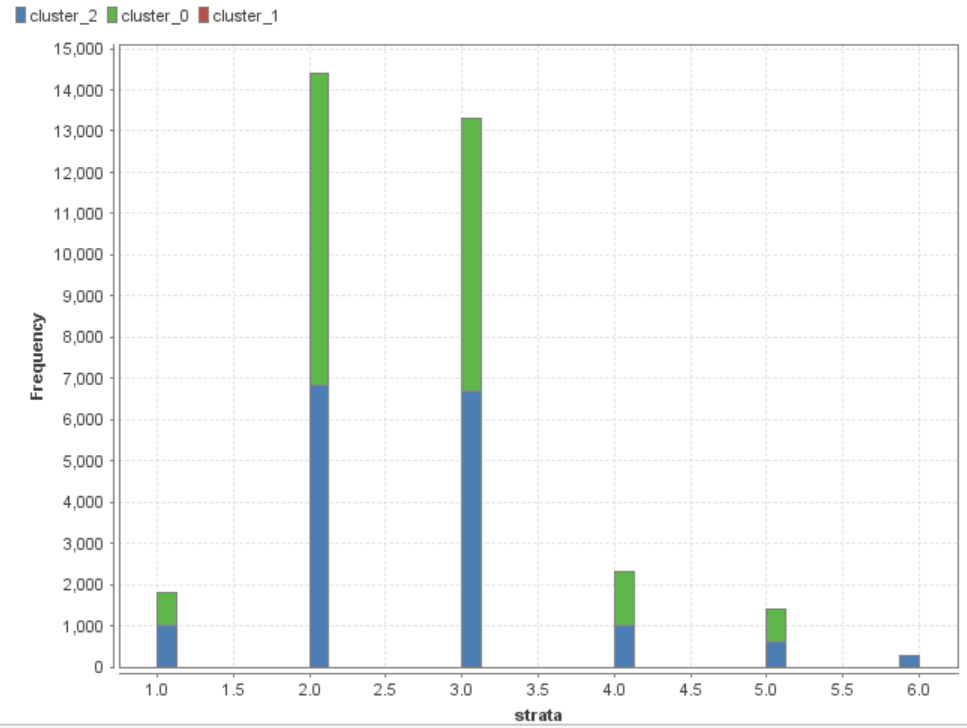
\includegraphics[width=0.69\textwidth]{vectorClustering31000.PNG}
\caption{1000 steps clustering in 3 clusters}
\label{fig:1000vect3}
\end{figure}

Figure \ref{fig:1000vect3} shows clearly, that again no correlation can be found. Furthermore we applied this for the different datasets we generated, but the result was always similar.


